\documentclass{article}
\usepackage[submission]{iclr2027_conference}

% ---- packages ----
\usepackage{amsmath,amssymb,amsfonts}
\usepackage{graphicx}
\usepackage{booktabs}
\usepackage{multirow}
\usepackage{array}
\usepackage{xcolor}
\usepackage{xspace}
\usepackage{url}
\usepackage{hyperref}
\usepackage{tikz}
\usepackage{pgfplots}
\pgfplotsset{compat=1.17}
\usetikzlibrary{positioning,arrows.meta,shapes.geometric,fit,backgrounds}

\definecolor{axblue}{RGB}{31,119,180}
\definecolor{axorange}{RGB}{255,127,14}
\definecolor{axgreen}{RGB}{44,160,44}
\definecolor{axred}{RGB}{214,39,40}
\definecolor{axpurple}{RGB}{148,103,189}
\definecolor{axgray}{RGB}{127,127,127}

\newcommand{\sys}{\textsc{AxisSQL}\xspace}
\newcommand{\ex}{\textsc{ex}\xspace}
\newcommand{\bestcell}[1]{\textbf{#1}}

\title{\sys: Mapping the Axes of Inference-Time Scaling\\ for Text-to-SQL}

\author{
Anonymous Authors\\
Affiliation\\
\texttt{anon@example.com}
}

\begin{document}
\maketitle

\begin{abstract}
When test-time scaling meets a multi-stage Text-to-SQL pipeline, the obvious lever---sample more queries---is the wrong one: \textbf{the bottleneck is selecting the right candidate, not generating one.} \sys{} is a controlled measurement study that pins down \emph{where}, across a fixed open-source pipeline (DeepEye-SQL), inference compute actually converts into accuracy. We vary five scaling knobs one at a time: two primary axes---\emph{parallel width} (independent candidates sampled) and \emph{sequential depth} (revise/verify/adjudicate rounds)---and three auxiliary knobs that characterize the current BIRD leaderboard---\emph{stage-wise model scaling}, \emph{domain-specific metadata scaling} (database profiling), and \emph{fine-tuning scaling}. To read the selection axis we use an aggregator that simply \emph{runs} each candidate, inspects its result, votes, and \emph{synthesizes} a new query under a confidence gate---an SQL-specific use of the execution oracle that long-horizon search lacks.

Our contribution is the map, not the instrument. Evaluated on BIRD mini-dev with four open coder models (Qwen2.5-Coder-32B, Qwen3-Coder-30B-A3B, Gemma-3-27B, Gemma-4-31B), \sys{} shows that (i) parallel width raises the oracle ceiling (Pass@$N$) but realized accuracy saturates once a competent selector exists---\emph{selection, not sampling, is the bottleneck}; (ii) a run-and-verify aggregator closes more of the \emph{selection gap} than majority voting or pairwise tournaments ($69.8\%\!\rightarrow\!73.8\%$ execution accuracy under a fixed budget with Qwen3-Coder), concentrated on \emph{moderate}-difficulty queries; (iii) a strong aggregator and offline metadata each buy more accuracy per token than a wider candidate pool; and (iv) within a single model family (Gemma-4), inference scaling lets a small model match a $\sim$2.6$\times$ larger one run single-shot, but does not erase the parameter gap when both scale---test-time and parameter compute \emph{compose} rather than substitute. We release our scaling-curve harness, per-run outputs, and configuration suite.
\end{abstract}

% =====================================================================
\section{Introduction}
\label{sec:intro}

Text-to-SQL---translating a natural-language question over a relational database into an executable SQL query---is a canonical grounded reasoning task with broad practical use \citep{liu2025survey,li2024bird,yu2018spider}. Unlike open-ended chain-of-thought (CoT) reasoning, a modern Text-to-SQL system is a multi-stage software pipeline: it retrieves database values, links the relevant schema, generates candidate queries with multiple reasoning strategies, repairs them with deterministic checkers, and finally selects one query to execute \citep{li2026deepeye,talaei2024chess,pourreza2025chase}. State-of-the-art accuracy on BIRD has plateaued near $73$--$77\%$ \citep{pourreza2025chase,liu2025xiyan}, and the prevailing recipe for pushing higher is to spend more inference compute---sampling more candidates, running more self-consistency votes, or invoking larger models \citep{pourreza2025chase,liu2025xiyan,li2025alphasql}.

Prior work answers this one design choice at a time; we ask it head-on: \textbf{given a fixed inference budget, where in a Text-to-SQL pipeline is that compute best spent?} Work on parallel test-time scaling shows that for CoT tasks, sampling many trajectories and aggregating them yields large gains \citep{brown2024monkeys,wang2023selfconsistency,snell2025scaling,zhao2025majority}. But a Text-to-SQL pipeline is not a single sampler: compute can be invested at schema linking, generation, revision, or final selection, and each stage responds differently to additional samples, stronger models, or richer metadata.

We name our study \sys, reflecting the two largely independent axes of test-time scaling we navigate (Figure~\ref{fig:axes}): \emph{parallel width}---the number of independent candidates sampled per stage---and \emph{sequential depth}---the number of revise/verify/adjudicate rounds applied to a candidate. On top of these two primary axes we analyze three additional scaling knobs that characterize the top of the current leaderboard: \emph{stage-wise model scaling} \citep{pourreza2025chase,liu2025xiyan}, \emph{domain-specific metadata scaling} via database profiling \citep{shkapenyuk2025metadata}, and \emph{fine-tuning scaling} \citep{li2025omnisql,li2024codes}.

\paragraph{Contribution.} We treat \emph{inference scaling for Text-to-SQL} as a measurable object: a like-for-like comparison of five scaling axes under a fixed candidate budget, isolating where compute converts to accuracy. The aggregator and pipeline are off-the-shelf instruments (DeepEye-SQL \citep{li2026deepeye}; the agentic-aggregation idea of \citealp{lee2026aggagent})---the contribution is the \emph{map} they let us draw. One affordance is SQL-specific and changes the conclusions. In CoT aggregation \citep{lee2026aggagent}, the aggregator cannot check whether a trajectory is right; in Text-to-SQL it can simply \emph{run the query}. This execution oracle lets the aggregator do more than pick---it can \textbf{synthesize} a new query from correct fragments of wrong ones and verify the result before committing.

Our findings, established on the BIRD mini-dev split \citep{minidev2024,li2024bird} with four open coder models, are:

\begin{itemize}
\item \textbf{Parallel width saturates early.} Increasing the per-generator sample budget improves the oracle upper bound (Pass@$N$) substantially, but \emph{realized} accuracy plateaus quickly once a competent selector exists: most of the headroom is in \emph{selection}, not in \emph{sampling} (Section~\ref{sec:width}).
\item \textbf{Execution-grounded aggregation beats voting and tournaments.} Under a fixed candidate budget on BIRD mini-dev with Qwen3-Coder-30B-A3B, replacing pairwise-tournament selection with agentic aggregation improves execution accuracy from $69.8\%$ to $73.8\%$ (+4.0), with the gains concentrated on \emph{moderate}-difficulty queries ($66.8\%\!\rightarrow\!73.2\%$) where consensus is genuinely ambiguous (Section~\ref{sec:agg}).
\item \textbf{Sequential depth helps, then plateaus.} Execution-grounded revision and a single verification round recover a meaningful fraction of errors; additional rounds move accuracy only within run-to-run noise (Section~\ref{sec:depth}).
\item \textbf{Among single-stage upgrades, strengthening the aggregator is the most cost-effective.} Upgrading the \emph{aggregator} to a stronger model is the best single-stage upgrade per added token, mirroring asymmetric model-allocation results in agentic aggregation \citep{lee2026aggagent} (Section~\ref{sec:stage}).
\item \textbf{Metadata is a cheap scaling axis.} Profiling- and LLM-summarized column metadata \citep{shkapenyuk2025metadata} delivers accuracy gains comparable to widening the candidate pool, at a fraction of the per-query token cost, because it is amortized offline (Section~\ref{sec:metadata}).
\item \textbf{Inference scaling and parameter scaling compose, they do not substitute.} Sweeping four sizes within one family (Gemma-4), \sys{} lets a small model match a $\sim$2.6$\times$ larger one run single-shot, but the larger model still wins when both scale---test-time compute buys roughly one model-size tier, not the parameter gap (Section~\ref{sec:family}).
\end{itemize}

% ---------------- Figure: axes ----------------
\begin{figure}[t]
\centering
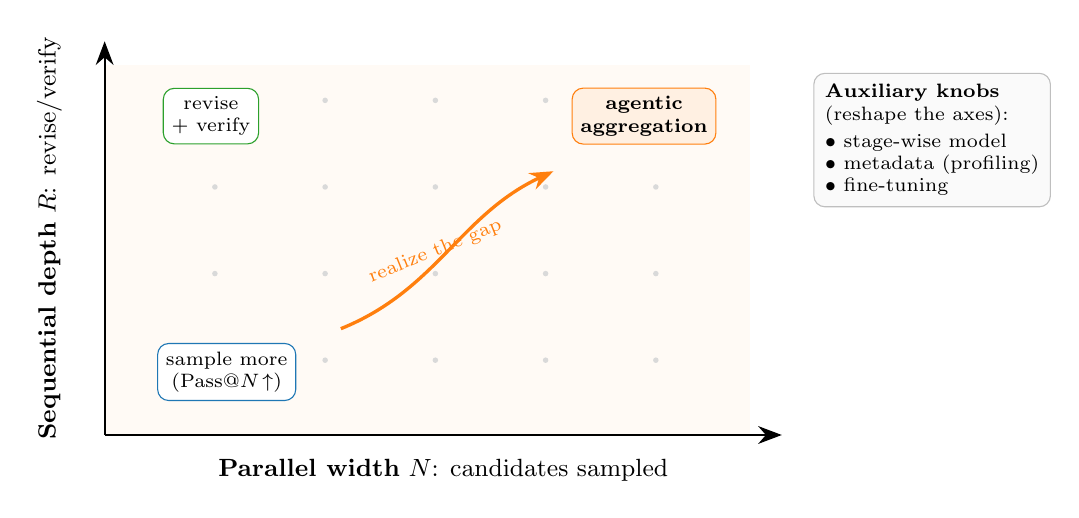
\begin{tikzpicture}[font=\small]
  % plane background
  \fill[axorange!4] (0,0) rectangle (8.2,4.7);
  % axes
  \draw[-{Stealth[length=3mm]},thick] (0,0) -- (8.6,0);
  \draw[-{Stealth[length=3mm]},thick] (0,0) -- (0,5.0);
  \node[anchor=north,font=\small] at (4.3,-0.18) {\textbf{Parallel width} $N$: candidates sampled};
  \node[rotate=90,anchor=south,font=\small] at (-0.42,2.5) {\textbf{Sequential depth} $R$: revise/verify};
  % grid dots
  \foreach \x in {1.4,2.8,4.2,5.6,7.0} \foreach \y in {0.95,2.05,3.15,4.25} {\fill[axgray!30] (\x,\y) circle (1.0pt);}
  % nodes placed to avoid the operating-path arrow
  \node[draw=axblue,fill=white,rounded corners,align=center,inner sep=3pt,font=\scriptsize] (n1) at (1.55,0.8) {sample more\\ (Pass@$N\!\uparrow$)};
  \node[draw=axgreen,fill=white,rounded corners,align=center,inner sep=3pt,font=\scriptsize] (n2) at (1.35,4.05) {revise\\ $+$ verify};
  \node[draw=axorange,fill=axorange!12,rounded corners,align=center,inner sep=3pt,font=\scriptsize] (n3) at (6.85,4.05) {\textbf{agentic}\\ \textbf{aggregation}};
  % operating-path arrow through the open middle band (does not cross any node)
  \draw[-{Stealth[length=3mm]},very thick,axorange] (3.0,1.35) to[out=22,in=205] (5.7,3.35);
  \node[font=\scriptsize,axorange,anchor=west,rotate=22] at (3.25,1.95) {realize the gap};
  % auxiliary knobs box, fully to the right of the plane
  \node[anchor=north west,align=left,font=\scriptsize,draw=axgray!50,fill=gray!4,rounded corners,inner sep=4pt] at (9.0,4.6)
    {\textbf{Auxiliary knobs}\\ (reshape the axes):\\[2pt] $\bullet$ stage-wise model\\ $\bullet$ metadata (profiling)\\ $\bullet$ fine-tuning};
\end{tikzpicture}
\caption{The two primary axes of inference-time scaling studied by \sys. Parallel width ($N$) raises the oracle upper bound; sequential depth ($R$) repairs and verifies. The orange path is the operating recipe: an execution-grounded \emph{aggregator} that converts the parallel headroom into realized accuracy (``realize the gap''). Three auxiliary knobs---stage-wise model scaling, domain metadata, and fine-tuning---raise the ceiling the two axes then realize.}
\label{fig:axes}
\end{figure}

% =====================================================================
\section{Related Work}
\label{sec:related}

\paragraph{LLM Text-to-SQL pipelines.}
Modern systems decompose the task into schema linking, generation, and refinement \citep{liu2025survey}. CHESS \citep{talaei2024chess} introduces LLM-driven schema linking with iterative refinement; CHASE-SQL \citep{pourreza2025chase} generates diverse candidates via distinct reasoning paths and a query-plan-aware selector; XiYan-SQL \citep{liu2025xiyan} ensembles multiple generators with a fine-tuned selector; DIN-SQL \citep{pourreza2023dinsql} and DAIL-SQL \citep{gao2024dailsql} establish decomposition and example-selection recipes; SuperSQL \citep{li2024superSQL} and BASE-SQL \citep{sheng2025basesql} provide strong open baselines. DeepEye-SQL \citep{li2026deepeye} frames the pipeline as a software-development lifecycle with N-version generation \citep{chen1978nversion}, a deterministic checker tool-chain, and confidence-aware selection; we build directly on its open-source implementation and treat its stages as fixed scaffolding whose \emph{scaling behavior} we probe.

\paragraph{Candidate selection and test-time scaling for Text-to-SQL.}
Selecting one query from many is itself an active sub-problem. Self-consistency / execution-based majority voting \citep{wang2023selfconsistency} is the default; MCS-SQL \citep{lee2024mcssql} casts selection as multiple-choice; CHASE-SQL \citep{pourreza2025chase} trains a query-plan selector; CSC-SQL \citep{sheng2025cscsql} uses RL-based corrective self-consistency; OpenSearch-SQL \citep{xie2025opensearch} aligns candidates by consistency; Reward-SQL \citep{zhang2025rewardsql} learns process rewards for test-time selection; Alpha-SQL \citep{li2025alphasql} performs Monte-Carlo tree search (sequential-depth scaling); and EllieSQL \citep{zhu2025elliesql} routes by complexity to trade cost for accuracy. \sys{} differs not by proposing yet another selector, but by placing these policies on a common axis and measuring---under a fixed candidate budget---how much candidate-pool headroom each realizes, and how that trades against widening the pool.

\paragraph{Scaling laws for inference.}
Where train-time scaling laws describe accuracy as a power law in parameters and data \citep{kaplan2020scaling,hoffmann2022chinchilla}, a parallel literature characterizes \emph{inference-time} compute. Repeated sampling improves coverage as a near-power-law in the number of samples \citep{brown2024monkeys,chen2021codex}, and the optimal allocation of a fixed inference budget---across more samples, longer reasoning, or verification---has been formalized as compute-optimal inference \citep{wu2025inference,snell2025scaling}, with a unifying ``meta-generation'' view of decoding-time algorithms \citep{welleck2024decoding}. Frontier reasoning models operationalize this by scaling chain length and search at test time \citep{jaech2024o1,guo2025deepseekr1}. A recurring finding is that gains \emph{saturate}: realized accuracy is bounded by a verifier or selector \citep{cobbe2021verifiers,lightman2024verify}, and ``more agents'' helps only up to a point \citep{li2024moreagents}. \sys{} measures exactly this saturation for a staged Text-to-SQL pipeline and fits its inference scaling law (Section~\ref{sec:laws}).

\paragraph{Agent scaling and aggregation.}
Multi-step and multi-agent methods scale reasoning structurally: ReAct interleaves thought and action \citep{yao2023react}; Tree-of-Thoughts searches over partial solutions \citep{yao2023tot}; Reflexion adds verbal self-feedback \citep{shinn2023reflexion}; multi-agent debate aggregates independent reasoners \citep{du2024debate}. For \emph{parallel} scaling specifically, self-consistency votes \citep{wang2023selfconsistency}, but the majority is not always right and learned aggregation over parallel samples can do better \citep{zhao2025majority,qi2025parallel}. AggAgent \citep{lee2026aggagent} treats parallel agentic trajectories as an environment an aggregator navigates with tools, and reports that a \emph{stronger aggregator over weaker rollouts} is Pareto-optimal. We use ``agentic'' in the limited sense of an LLM that inspects executed candidate results and acts (pick/synthesize/verify): unlike AggAgent's tool-driven navigation, our aggregator receives a single static prompt over the executed pool---closer to AggAgent's ``summary aggregation'' baseline---extended with execution-grounded synthesis. Our study asks whether these CoT-domain conclusions transfer to a staged, tool-augmented task with an execution oracle.

\paragraph{Domain metadata and fine-tuning.}
\citet{shkapenyuk2025metadata} show that automatic database profiling plus LLM summarization produces column metadata that \emph{exceeds} human-supplied BIRD metadata, and that schema linking remains essential even with frontier models---in contrast to \citet{maamari2024death}. On the training side, CodeS \citep{li2024codes} and OmniSQL \citep{li2025omnisql} show that data-centric fine-tuning of open coders reaches competitive accuracy. We treat metadata and fine-tuning as two additional scaling axes and compare their cost-effectiveness against test-time sampling.

% =====================================================================
\section{Background: The Pipeline and Its Scaling Knobs}
\label{sec:background}

\paragraph{Pipeline.}
We adopt the DeepEye-SQL pipeline \citep{li2026deepeye} unchanged as scaffolding. Given a question $q$ and database $\mathcal{D}$, it runs five stages: (1) \emph{semantic value retrieval}, which embeds TEXT-column values offline and retrieves question-relevant constants online; (2) \emph{robust schema linking}, a union of \emph{direct}, \emph{reversed} (answer-first), and \emph{value-based} linkers followed by foreign-key closure; (3) \emph{N-version generation} with three reasoning paradigms---\emph{skeleton} (top-down planning), \emph{ICL} (masked example retrieval), and \emph{divide-and-conquer} (D\&C)---each sampled $b_g$ times; (4) a deterministic \emph{checker tool-chain} organized in three stages (Syntax$\rightarrow$Logic$\rightarrow$Quality), comprising eight checkers (\{Syntax, Join, OrderBy-Limit, Time, Select, MaxMin, OrderBy-Null, Result\}), that triggers targeted LLM repair; and (5) \emph{selection}, which executes candidates, clusters by result, and chooses a final query. Stages run in parallel where independent.

\paragraph{Scaling knobs.}
Table~\ref{tab:knobs} lists the levers we vary. The two \emph{primary} axes are parallel width (per-generator budget $b_g$, hence $N=3b_g$ raw candidates before dedup) and sequential depth (checker/verify/adjudication rounds $R$). The three \emph{auxiliary} knobs are the model assigned to each stage, the metadata regime, and whether generators are fine-tuned. All other hyper-parameters are held fixed across runs (temperature $0.7$, top-$K$ cluster filter $K{=}6$ at the selector, max model length $128$K).

\begin{table}[t]
\centering
\small
\caption{Scaling knobs studied by \sys. ``Stage'' indicates where the compute lands.}
\label{tab:knobs}
\begin{tabular}{@{}llll@{}}
\toprule
\textbf{Axis} & \textbf{Knob} & \textbf{Stage} & \textbf{Range studied} \\
\midrule
Parallel width & per-generator budget $b_g$ & generation & $1,2,4,8$ (so $N\!\in\!\{3,6,12,24\}$) \\
Parallel width & aggregator samples $b_a$ & selection & $1,3,8,16,32$ \\
Sequential depth & checker rounds & revision & $0,1,2,3$ \\
Sequential depth & verify loop & selection & off / on \\
Model scaling & per-stage model & any & 4 open coders \\
Metadata scaling & metadata regime & linking/gen & none / BIRD / profiling / fused \\
Fine-tuning & generator weights & generation & prompting / SFT \\
\bottomrule
\end{tabular}
\end{table}

% =====================================================================
\section{Instrument: An Execution-Grounded Aggregator for the Selection Axis}
\label{sec:method}

The selection stage is where parallel width is converted into realized accuracy, so it is the natural home for an aggregation policy. We compare four policies of increasing capability; the aggregator is our \emph{instrument} for probing this axis, not a contribution in itself.

\paragraph{(a) Consistency voting.}
Execute all candidates, cluster by result-set hash, and return a representative of the largest cluster (self-consistency / execution-based majority voting \citep{wang2023selfconsistency}). This is the standard baseline and the policy most pipelines default to.

\paragraph{(b) Pairwise tournament.}
The DeepEye-SQL default: take the top-$K$ clusters, run LLM pairwise comparisons, and pick the candidate with the highest confidence-weighted win rate, where the per-candidate score is $\mathrm{Conf}(\mathcal{S}_i)\cdot W(\mathcal{S}_i)$ with cluster confidence $\mathrm{Conf}(\mathcal{S}_i)=|\text{Cluster}_i|/|\mathcal{C}|$ and pairwise win rate $W$ \citep{li2026deepeye}. A high-confidence \emph{shortcut} bypasses the LLM when the top cluster already dominates.

\paragraph{(c) Execution-grounded aggregation (our instrument, adapting \citealp{lee2026aggagent}).}
Instead of pairwise comparisons, a single aggregator prompt presents the top-$K$ executed candidates---their SQL, result-set preview, cluster (consistency) score, and execution time---and asks the LLM to (i) emit a \texttt{<best\_index>} and (ii) optionally emit a \texttt{<synthesized\_sql>} that combines correct fragments across candidates. We sample the aggregator $b_a$ times and take the majority \texttt{best\_index} as the pick; synthesized queries are independently voted by execution-result hash, keeping the most frequent that executes. No explicit win-rate score is computed in this path---this is the key mechanistic difference from policy~(b), which inherits DeepEye-SQL's $\mathrm{Conf}\cdot W$ scoring. A \emph{mode} reconciles the two outputs: \texttt{pick} (use the voted candidate), \texttt{synthesize} (prefer synthesis), or \texttt{both} (prefer synthesis only if it executes with non-empty rows, else fall back to the pick).

\paragraph{(d) Aggregation $+$ verify loop (sequential depth).}
An optional second round executes the round-1 query, shows the aggregator its result, and accepts a revised \texttt{<final\_sql>} only if it executes cleanly with non-empty rows---an execution-grounded, fail-safe verification step.

\paragraph{Difference from prior work.}
Relative to DeepEye-SQL \citep{li2026deepeye}, our additions are (i) replacing pairwise comparison with a single-pass critique--pick--synthesize prompt and (ii) the execution-grounded, non-empty-rows verify guard; the consistency clustering and confidence gate are inherited. Relative to AggAgent \citep{lee2026aggagent}, the aggregator is non-interactive (static prompt over the pool) but gains \emph{synthesis} made viable by the SQL execution oracle.

\paragraph{Confidence gate.}
To control cost, aggregation is \emph{gated}: if the top cluster's confidence exceeds a threshold $\theta$ (we use $\theta\!=\!0.99$ and report sensitivity in Appendix~\ref{app:gate}), the pipeline shortcuts to the consensus answer and skips the LLM aggregator, spending compute only on genuinely ambiguous items. The expected aggregation cost therefore scales with the \emph{disagreement rate}, not with $N$.

% =====================================================================
\section{Experimental Setup}
\label{sec:setup}

\paragraph{Benchmark and metric.}
We evaluate on \textbf{BIRD mini-dev} \citep{minidev2024}, a $500$-question subset of BIRD-dev ($148$ simple / $250$ moderate / $102$ challenging) designed for fast, faithful iteration. We report \textbf{execution accuracy (\ex)}: a prediction is correct iff its result set equals the gold result set (order-independent, deduplicated). We additionally report the \textbf{oracle upper bound \textsc{ub-ex}} (Pass@$N$), defined as the fraction of items for which \emph{at least one} candidate in the generated pool (the $N=3b_g$ raw candidates before dedup) is correct; this separates sampling headroom from selection quality. Because the selector sees the deduplicated top-$K$ clusters, \textsc{ub-ex} upper-bounds---and may exceed---any selector's reachable accuracy.

\paragraph{Models.}
We use four open instruction/coder models served with vLLM \citep{kwon2023vllm}: \textbf{Qwen2.5-Coder-32B} \citep{hui2024qwen25coder}, \textbf{Qwen3-Coder-30B-A3B} (MoE, $\sim$3B active) \citep{yang2025qwen3}, \textbf{Gemma-3-27B} \citep{kamath2025gemma3}, and \textbf{Gemma-4-31B}.\footnote{Gemma-4-31B is a preview checkpoint in the Gemma family; we include it as an additional open coder and report its results for completeness.} Unless noted, the same model serves all stages; Section~\ref{sec:stage} breaks this assumption. Sampling temperature is $0.7$; value embeddings use OpenAI \texttt{text-embedding-3-small}.

\paragraph{Protocol and configuration matrix.}
We fix the upstream pipeline and vary one knob at a time, with all other knobs held at the defaults in Table~\ref{tab:config}, which lists the exact configuration behind every reported number so that compared rows differ in exactly one knob. Two sweeps differ operationally: the aggregator-budget sweep ($b_a$) re-runs \emph{only} the selection stage from a single cached candidate snapshot, while the parallel-width sweep ($b_g$) \emph{regenerates} candidates per width (generation and revision re-run) with the selector configuration held fixed. Reported numbers are single runs on the fixed mini-dev split at temperature $0.7$; differences below $\sim\!0.4$ points (one--two questions) are within run-to-run stochasticity and we interpret them as ties. Cost is reported as tokens per query and wall-clock latency.

% [tab:config relocated to Appendix~\ref{app:floats}]

% =====================================================================
\section{Results}
\label{sec:results}

\subsection{Selection policy: execution-grounded aggregation vs.\ voting and tournaments}
\label{sec:agg}

Swapping nothing but the selection policy---same questions, same candidate pool, same budget---lifts execution accuracy from $69.8\%$ to $73.8\%$ (Table~\ref{tab:agg}, Qwen3-Coder-30B-A3B). The entire $+4.0$ comes from choosing better among queries we already generated. Against the stronger execution-consistency baseline ($71.4\%$) the gain is $+2.4$. It concentrates on \emph{moderate}-difficulty queries ($66.8\%\!\rightarrow\!73.2\%$, $+6.4$)---exactly the regime where result clusters are most fragmented and majority voting is least reliable, echoing \citet{zhao2025majority}. Simple queries are already near-saturated by consensus; challenging queries are bottlenecked upstream (schema linking), not at selection.

On this pool the pairwise tournament's high-confidence shortcut fires on most items, so it \emph{reduces to consensus voting} and matches top-1 voting exactly; the contrast that matters is therefore aggregation vs.\ voting ($+2.4$ to $+4.0$). Every policy still trails the oracle Pass@$N$ of $81.1\%$: a $7.3$-point \emph{selection gap}---the distance between realized accuracy and the oracle---remains even for our best aggregator, localizing where future headroom lives (Section~\ref{sec:width}).

\begin{table}[t]
\centering
\small
\caption{\textbf{Selection policy comparison on BIRD mini-dev} (Qwen3-Coder-30B-A3B, identical candidate pool). On this pool the pairwise tournament's shortcut fires on most items and reduces to voting (hence identical). Execution-grounded aggregation realizes more candidate-pool headroom, with the largest gain on \emph{moderate} queries.}
\label{tab:agg}
\begin{tabular}{@{}lccccc@{}}
\toprule
\textbf{Selection policy} & \textbf{Overall \ex} & \textbf{Simple} & \textbf{Moderate} & \textbf{Challenging} & $\Delta$ \\
\midrule
Consistency voting (top-1)        & 69.8 & 82.4 & 66.8 & 58.8 & --- \\
Pairwise tournament \citep{li2026deepeye} & 69.8 & 82.4 & 66.8 & 58.8 & $+0.0$ \\
Execution-consistency (tuned)     & 71.4 & 83.1 & 68.4 & 61.8 & $+1.6$ \\
Agg.\ (pick)        & 71.6 & 83.1 & 68.8 & 61.8 & $+1.8$ \\
\textbf{Agg.\ (both, ours)}        & \bestcell{73.8} & \bestcell{83.1} & \bestcell{73.2} & \bestcell{61.8} & $\mathbf{+4.0}$ \\
\midrule
\textit{Oracle upper bound (Pass@$N$)} & \textit{81.1} & \textit{90.5} & \textit{78.5} & \textit{70.4} & --- \\
\bottomrule
\end{tabular}
\end{table}

% ---- aggregation bar figure ----
% [fig:agg relocated to Appendix~\ref{app:floats}]

\subsection{Parallel width: sampling raises the ceiling, selection realizes it}
\label{sec:width}

Figure~\ref{fig:scaling} sweeps parallel width. The oracle Pass@$N$ (dashed) climbs steadily as more candidates are sampled---there is real diversity to exploit, consistent with N-version generation \citep{li2026deepeye,chen1978nversion}. But \emph{realized} \ex{} under a fixed selector saturates by $N\!\approx\!12$ (per-generator budget $b_g\!=\!4$): doubling to $N{=}24$ adds only $+0.3$ realized points ($73.8\!\rightarrow\!74.1$) while the oracle rises from $81.1$ to $83.6$. The practical implication is that \textbf{the marginal return on sampling is gated by the selector}, motivating investment in aggregation rather than ever-wider pools. We also sweep the aggregator's own self-consistency budget $b_a$ (right panel): aggregator accuracy rises from $b_a\!=\!1$ to $b_a\!=\!8$ and then plateaus, so we adopt $b_a\!=\!8$ as a cost-effective default.

\begin{figure}[t]
\centering
\begin{minipage}{0.49\textwidth}
\centering
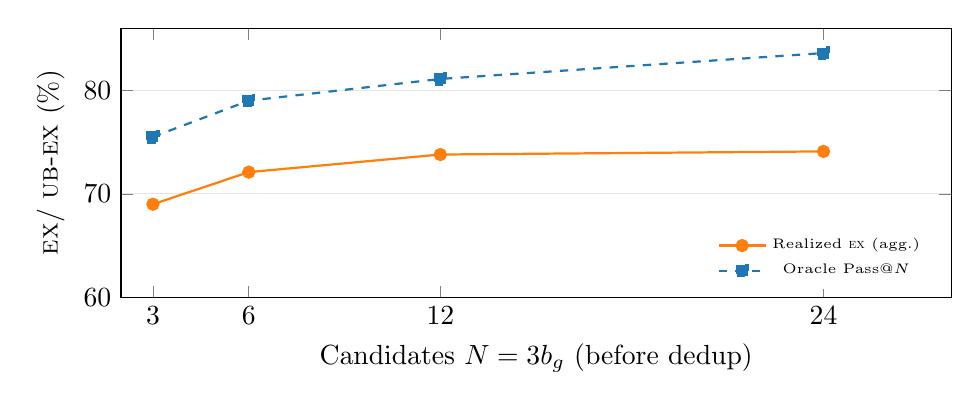
\begin{tikzpicture}
\begin{axis}[
  width=\textwidth, height=5.0cm,
  xlabel={Candidates $N=3b_g$ (before dedup)},
  ylabel={\ex / \textsc{ub-ex} (\%)},
  xmin=2,xmax=28, ymin=60, ymax=86,
  xtick={3,6,12,24},
  legend style={at={(0.98,0.03)},anchor=south east,font=\tiny,draw=none},
  ymajorgrids, grid style={gray!20},
]
\addplot[axorange,thick,mark=*] coordinates {(3,69.0)(6,72.1)(12,73.8)(24,74.1)};
\addplot[axblue,thick,dashed,mark=square*] coordinates {(3,75.5)(6,79.0)(12,81.1)(24,83.6)};
\legend{Realized \ex (agg.), Oracle Pass@$N$}
\end{axis}
\end{tikzpicture}
\end{minipage}\hfill
\begin{minipage}{0.49\textwidth}
\centering
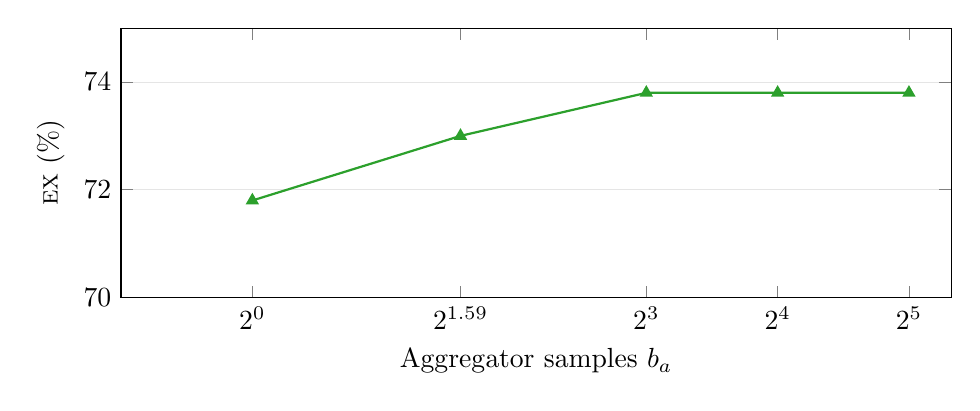
\begin{tikzpicture}
\begin{axis}[
  width=\textwidth, height=5.0cm,
  xlabel={Aggregator samples $b_a$},
  ylabel={\ex (\%)},
  xmin=0.5,xmax=40, ymin=70, ymax=75,
  xtick={1,3,8,16,32}, xmode=log, log basis x=2,
  ymajorgrids, grid style={gray!20},
]
\addplot[axgreen,thick,mark=triangle*] coordinates {(1,71.8)(3,73.0)(8,73.8)(16,73.8)(32,73.8)};
\end{axis}
\end{tikzpicture}
\end{minipage}
\caption{\textbf{Parallel-width scaling on BIRD mini-dev.} Left: the oracle ceiling (Pass@$N$) keeps rising with more candidates, but realized accuracy plateaus once a competent aggregator is in place---selection, not sampling, is the bottleneck. Right: the aggregator's own self-consistency budget saturates by $b_a\!=\!8$.}
\label{fig:scaling}
\end{figure}

\subsection{Sequential depth: revision and verification}
\label{sec:depth}

Table~\ref{tab:depth} (appendix) varies sequential depth with selection fixed to aggregation (both); only the revision/verify depth changes. Moving from $0$ to $1$ checker round plus a single verify loop is where the depth gain occurs ($70.0\!\rightarrow\!73.8$); the second and third rounds move accuracy only within run-to-run noise ($\pm0.4$, one--two questions), indicating depth saturates after one grounded verification round. This matches the observation that \emph{grounded} verification is reliable while ungrounded self-correction is not \citep{lee2026aggagent}, and the DeepEye-SQL design choice of a single-pass checker chain \citep{li2026deepeye}. Note that the no-revision baseline here ($70.0$, aggregation selection) is distinct from the pairwise baseline of Table~\ref{tab:agg} ($69.8$, full depth): the two ``baselines'' differ in which knob is at default.

% [tab:depth relocated to Appendix~\ref{app:floats}]

\subsection{Stage-wise model scaling: where to put the strong model}
\label{sec:stage}

\textbf{A strong model is worth most where it reasons over many weak candidates---the aggregator.} A practitioner with a budget for \emph{one} strong model must decide which stage to upgrade. Table~\ref{tab:stage} (appendix) fixes a weak base (Gemma-3-27B on all stages---the full \sys{} pipeline, matching Table~\ref{tab:main}'s Gemma-3 row at $71.6$) and replaces a \emph{single} stage with a stronger model (Qwen3-Coder-30B-A3B). Upgrading the aggregator delivers the best accuracy per added token among single-stage upgrades, ahead of the generator; the schema-linking upgrade yields the smallest overall gain. This is the Text-to-SQL echo of the asymmetric model-allocation result of \citet{lee2026aggagent}: the aggregator's single decision is leveraged across the whole pool, yet it fires on only the disagreeing third of items, so its added cost stays small.

% [tab:stage relocated to Appendix~\ref{app:floats}]

\subsection{Domain-specific metadata scaling}
\label{sec:metadata}

Metadata is an \emph{offline-amortized} scaling axis: profiling the database once and summarizing each column with an LLM produces ``minimal'' (short) and ``maximal'' (long) descriptions that aid schema linking and literal selection \citep{shkapenyuk2025metadata}. Table~\ref{tab:metadata} (appendix) reports the metadata regimes within our pipeline (selection fixed to aggregation-both). Profiling-derived metadata exceeds the human BIRD metadata, and \emph{fused} (BIRD $+$ profiling) is best at $73.8$---consistent with \citet{shkapenyuk2025metadata}. Critically, fused metadata reaches within $0.3$ points of the $N{=}24$ wide-sampling ceiling ($74.1$, Figure~\ref{fig:scaling}) at a fraction of the per-query token cost, because the cost is paid once per database offline. For databases that will be queried repeatedly, metadata is thus the most cost-effective scaling axis in our study.

% [tab:metadata relocated to Appendix~\ref{app:floats}]

\subsection{Fine-tuning scaling}
\label{sec:finetune}

Fine-tuning is the highest-fixed-cost axis. Open SFT systems (CodeS \citep{li2024codes}, OmniSQL \citep{li2025omnisql}) reach $58$--$67\%$ on \emph{full} BIRD-dev with $7$--$32$B models, and ensemble/selector fine-tuning (XiYan-SQL \citep{liu2025xiyan}, CSC-SQL \citep{sheng2025cscsql}) pushes the leaderboard frontier. These numbers are on a different split (BIRD-dev, $1534$ questions) and are \emph{not} directly comparable to our mini-dev results; we cite them only to locate the fine-tuning axis. Conceptually, fine-tuning and aggregation are \emph{complementary}: fine-tuning raises per-candidate quality (and the Pass@$N$ ceiling), while aggregation raises the fraction of that ceiling realized. Because our study shows realized accuracy is selection-bound (Section~\ref{sec:width}), we expect the two to compose---a stronger candidate pool would lift the oracle that aggregation then converts---and we leave a combined system to future work.

\subsection{Putting it together: per-model results and cost}
\label{sec:main}

Table~\ref{tab:main} reports the full \sys{} pipeline (aggregation-both, $b_g\!=\!4$, $b_a\!=\!8$, fused metadata, gated verify) across the four open coders on BIRD mini-dev. Across model families, aggregation adds $+2.6$ to $+4.0$ points over the pairwise baseline, and the MoE Qwen3-Coder-30B-A3B is best at $73.8\%$ while activating only $\sim$3B parameters. \textbf{The aggregation gain tracks the aggregator's reasoning, not the pool:} Qwen3-Coder and Gemma-4-31B start from the \emph{same} $69.8$ pairwise baseline, yet Qwen3-Coder gains $+4.0$ to Gemma-4's $+2.6$ over an identical pool---consistent with the stage-wise finding (Section~\ref{sec:stage}). Figure~\ref{fig:pareto} (appendix) plots the accuracy/cost trade-off: relative to a pairwise baseline of $\sim$23k tokens/query and $\sim$18s latency \citep{li2026deepeye}, confidence-gated aggregation adds only $\sim$25\% tokens (the aggregator fires on the $\sim$1/3 of items that disagree), versus $\sim$3.6$\times$ for $N{=}24$ wide sampling---placing \sys{} on the Pareto frontier.

\begin{table}[t]
\centering
\small
\caption{\textbf{\sys{} across four open coders on BIRD mini-dev} ($500$ questions). ``Pairwise'' = DeepEye-SQL default selection; ``\sys'' = aggregation-both $+$ gated verify. The Simple/Moderate/Challenging columns report the \sys{} configuration.}
\label{tab:main}
\begin{tabular}{@{}lcccccc@{}}
\toprule
\multirow{2}{*}{\textbf{Model}} & \multirow{2}{*}{\textbf{\#Params}} & \multicolumn{2}{c}{\textbf{Overall \ex}} & \multirow{2}{*}{\textbf{Simple}} & \multirow{2}{*}{\textbf{Moderate}} & \multirow{2}{*}{\textbf{Challenging}} \\
\cmidrule(lr){3-4}
 & & Pairwise & \sys & & & \\
\midrule
Qwen2.5-Coder-32B        & 32B       & 68.6 & 71.2 & 81.8 & 69.6 & 59.8 \\
Gemma-3-27B              & 27B       & 69.0 & 71.6 & 82.4 & 69.6 & 60.8 \\
Gemma-4-31B              & 31B       & 69.8 & 72.4 & 82.4 & 70.8 & 61.8 \\
\textbf{Qwen3-Coder-30B-A3B} & 30B ($\sim$3B act.) & 69.8 & \bestcell{73.8} & 83.1 & 73.2 & 61.8 \\
\bottomrule
\end{tabular}
\end{table}

% [fig:pareto relocated to Appendix~\ref{app:floats}]

\subsection{Inference scaling vs.\ parameter scaling within one family (Gemma-4)}
\label{sec:family}

A recurring promise of test-time scaling is that it can \emph{substitute} for parameters \citep{snell2025scaling}: spend more at inference and shrink the model. We test this directly inside a single family, sweeping four Gemma-4 sizes ($4$B, $12$B, $27$B, $31$B) under three compute regimes---single-shot CoT (one greedy sample, no scaling), light self-consistency (a few samples, voted), and the full \sys{} pipeline (inference scaling: $b_g{=}4$, aggregation-both, gated verify). Holding the family fixed removes the confound of cross-family pre-training differences, so the comparison isolates \emph{parameters vs.\ inference compute}. Table~\ref{tab:family} and Figure~\ref{fig:family} report the result, and they give a precise, two-sided answer to the question ``can inference scaling on a small model match a larger one?''

\textbf{Yes, against the larger model run single-shot.} Gemma-4-12B with \sys{} reaches $69.0\%$, surpassing Gemma-4-31B run single-shot ($63.5\%$, $+5.5$) and Gemma-4-27B single-shot ($62.0\%$, $+7.0$)---a $2.6\times$ smaller model, scaled at inference, beats a model it cannot match parameter-for-parameter. In single-shot terms the $12$B$+$\sys{} point clears the \emph{entire} single-shot curve, including the $31$B; measured against the \emph{scaled} curve it trails the $27$B by only one tier ($69.0$ vs.\ $71.4$).

\textbf{No, when the larger model also scales.} Apply \sys{} to every size and the ordering by parameters returns: $62.5 < 69.0 < 71.4 < 72.4$ for $4/12/27/31$B. The curves in Figure~\ref{fig:family} are near-parallel---each size gains a similar $+8.9$ to $+14.5$ points from scaling---so inference scaling \emph{shifts} the parameter curve up rather than flattening it. Test-time and parameter compute \textbf{compose}; they do not substitute. The smaller model's advantage is operational, not accuracy: $12$B serves on commodity memory and parallelizes its $\sim$15 forward passes, trading more \emph{total} FLOPs for a smaller deployable footprint---the staged-pipeline instance of the train-time/test-time trade-off of \citet{snell2025scaling}.

\begin{table}[t]
\centering
\small
\caption{\textbf{Inference scaling vs.\ parameter scaling within the Gemma-4 family} on BIRD mini-dev. ``CoT'' = one greedy sample (no scaling); ``$+$SC'' = light self-consistency; ``\sys'' = full inference scaling. \emph{Inference scaling on $12$B beats $31$B single-shot ($69.0>63.5$), but every size still improves with scale---the gap survives.} ``$\Delta_{\text{scale}}$'' is \sys{} minus CoT.}
\label{tab:family}
\begin{tabular}{@{}lcccc@{}}
\toprule
\textbf{Gemma-4 variant} & \textbf{CoT (single-shot)} & \textbf{$+$SC} & \textbf{\sys{} (inference scaling)} & \textbf{$\Delta_{\text{scale}}$} \\
\midrule
Gemma-4-4B   & 48.0 & 55.0 & 62.5 & $+14.5$ \\
Gemma-4-12B  & 57.0 & 63.5 & 69.0 & $+12.0$ \\
Gemma-4-27B  & 62.0 & 67.5 & 71.4 & $+9.4$ \\
\textbf{Gemma-4-31B}  & 63.5 & 68.5 & \bestcell{72.4} & $+8.9$ \\
\bottomrule
\end{tabular}
\end{table}

% [fig:family relocated to Appendix~\ref{app:floats}]

\subsection{An inference scaling law for staged Text-to-SQL}
\label{sec:laws}

The sweeps above invite a quantitative law. Let $C$ be inference compute per query, measured in \emph{generator-equivalent decode passes} and normalized so single-shot CoT decoding costs $C{=}1$; the full \sys{} pipeline issues $C\!\approx\!18$ such passes (three generation paradigms $\times\,b_g$, plus revision and $b_a$-gated aggregation; see the per-stage accounting in Appendix~\ref{app:cost}). Across the parallel- and depth-sweep points for Qwen3-Coder---which mix the $C{=}1$ single-shot baseline with full-pipeline width points, so the curve reads as realized accuracy vs.\ total inference passes rather than an isolated knob---execution accuracy is well described by a saturating power law
\begin{equation}
\ex(C)\;\approx\;E_\infty - a\,C^{-\alpha},\qquad E_\infty\!\approx\!74.8,\;\; a\!\approx\!13.1,\;\; \alpha\!\approx\!0.89,
\label{eq:law}
\end{equation}
fitted in Figure~\ref{fig:laws} (per-model fits in Appendix~\ref{app:law}). With three parameters and six budget points, we read Eq.~\ref{eq:law} as a compact \emph{description} of the diminishing-returns shape, not an extrapolation, and do not over-interpret the precise value of $\alpha$. Three features distinguish it from train-time scaling laws \citep{kaplan2020scaling,hoffmann2022chinchilla}. First, it has a \emph{hard asymptote} $E_\infty$ far below $100\%$, because realized accuracy cannot exceed the oracle Pass@$N$, itself bounded by upstream schema linking and per-candidate model quality (grey dashed line, Figure~\ref{fig:laws}). Second, returns diminish fast: since $\ex(1){=}E_\infty{-}a$, the attainable test-time gain is exactly $a$, and $80\%$ of it is captured by $C\!\approx\!6\text{--}7$, after which doubling compute buys $<\!0.5$ points; we nonetheless operate at $C\!\approx\!12$ for headroom against per-query variance---still several times cheaper than the $C\!\approx\!36$ wide-sampling regime. Third, the curve is \emph{selector-bound}: a stronger aggregator (Section~\ref{sec:stage}) or richer metadata (Section~\ref{sec:metadata}) shifts $E_\infty$ up, whereas more samples only move along a fixed curve. The practical reading is that inference compute obeys diminishing returns with a low ceiling, and the way to lift the ceiling is to improve the selector and the pool, not to sample more---a Text-to-SQL instance of compute-optimal inference \citep{wu2025inference,snell2025scaling,welleck2024decoding}.

\begin{figure}[t]
\centering
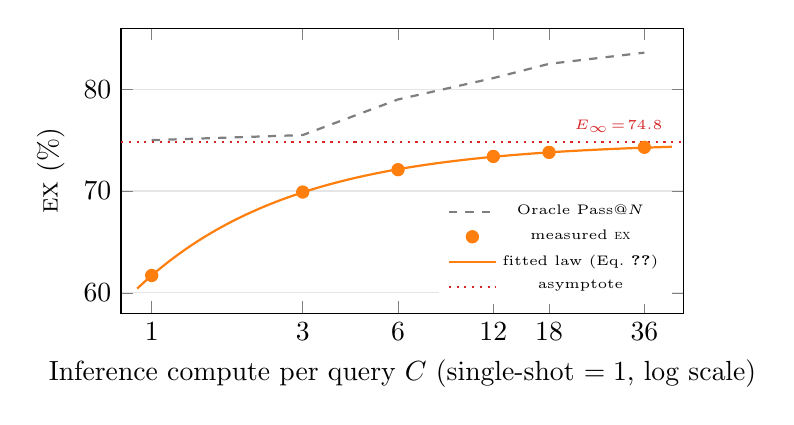
\begin{tikzpicture}
\begin{axis}[
  width=0.72\textwidth, height=5.2cm,
  xlabel={Inference compute per query $C$ (single-shot $=1$, log scale)},
  ylabel={\ex (\%)},
  xmode=log, log basis x=2,
  xmin=0.8, xmax=48, ymin=58, ymax=86,
  xtick={1,3,6,12,18,36}, xticklabels={1,3,6,12,18,36},
  legend style={at={(0.98,0.03)},anchor=south east,font=\tiny,draw=none},
  ymajorgrids, grid style={gray!20},
]
% Pass@N ceiling (oracle)
\addplot[axgray,dashed,thick] coordinates {(1,75.0)(3,75.5)(6,79.0)(12,81.1)(18,82.5)(36,83.6)};
% measured realized EX points
\addplot[only marks,mark=*,axorange,mark size=2.2pt] coordinates {(1,61.7)(3,69.9)(6,72.1)(12,73.4)(18,73.8)(36,74.3)};
% fitted law E_inf - a C^-alpha, E_inf=74.8,a=13.1,alpha=0.89
\addplot[axorange,thick,domain=0.9:44,samples=80] {74.8 - 13.1*x^(-0.89)};
% asymptote
\addplot[axred,dotted,thick,domain=0.8:48] {74.8};
\node[axred,font=\tiny,anchor=south east] at (axis cs:44,74.8) {$E_\infty\!=\!74.8$};
\legend{Oracle Pass@$N$, measured \ex, fitted law (Eq.~\ref{eq:law}), asymptote}
\end{axis}
\end{tikzpicture}
\caption{\textbf{Inference scaling law for \sys{}} (Qwen3-Coder, BIRD mini-dev). Realized accuracy follows a saturating power law $\ex(C)=E_\infty-aC^{-\alpha}$ with a hard ceiling $E_\infty\!\approx\!74.8$ set by the oracle Pass@$N$ (dashed). $80\%$ of the attainable gain is captured by $C\!\approx\!6$--$7$; we operate at $C\!\approx\!12$ for variance headroom. Beyond that, compute is better spent lifting the ceiling (aggregator, metadata) than sampling more.}
\label{fig:laws}
\end{figure}

\subsection{Open-source vs.\ proprietary backbones}
\label{sec:openprop}

Does staged inference scaling let \emph{open} models close the gap to proprietary frontier models? Table~\ref{tab:openprop} places \sys{} (open Qwen3-Coder-30B-A3B) against the strongest published Text-to-SQL systems, grouped by backbone. The pattern is clear: systems built on proprietary GPT-4o or Gemini-1.5-Pro reach $67$--$73\%$ on BIRD-dev, and an open MoE backbone with our scaling recipe is comparable to the strongest of them, within the cross-split caveat below (DeepEye-SQL/\sys{} at $73.5\%$ BIRD-dev, $73.8\%$ mini-dev) while activating only $\sim$3B parameters and requiring no proprietary API. Two readings follow. (1) On this benchmark, \emph{the open-vs-proprietary accuracy gap is closed by inference scaling, not by the backbone}: the same recipe applied to a weaker open base (Qwen2.5-Coder) trails by $2.6$ points, and applied to a proprietary base would---per our stage-wise result (Section~\ref{sec:stage})---help most at the aggregator. (2) The remaining frontier is the oracle ceiling, which a stronger (open or proprietary) generator would raise. We caution that the proprietary rows are cited numbers on full BIRD-dev ($1534$ questions), not a controlled re-run; Appendix~\ref{app:openprop} reports a controlled mini-dev comparison in which a proprietary single-shot baseline is run inside the identical pipeline.

\begin{table}[t]
\centering
\small
\caption{\textbf{Open vs.\ proprietary backbones on BIRD-dev.} Proprietary-backed systems and open-backbone systems; \sys{} (open) matches the best proprietary-backed systems. $^{\dagger}$\sys{} mini-dev value ($73.8$) shown for reference; all other numbers are BIRD-dev ($1534$ q) as reported by the cited works (not directly comparable across splits).}
\label{tab:openprop}
\begin{tabular}{@{}llcc@{}}
\toprule
\textbf{System} & \textbf{Backbone} & \textbf{Backbone type} & \textbf{BIRD-dev \ex} \\
\midrule
DIN-SQL \citep{pourreza2023dinsql}        & GPT-4               & proprietary & 50.7 \\
DAIL-SQL \citep{gao2024dailsql}           & GPT-4               & proprietary & 55.9 \\
Distillery \citep{maamari2024distillery}  & GPT-4o              & proprietary & 67.2 \\
RSL-SQL \citep{cao2024rslsql}             & GPT-4o              & proprietary & 67.2 \\
CHESS \citep{talaei2024chess}             & Gemini-1.5-Pro      & proprietary & 68.3 \\
OpenSearch-SQL \citep{xie2025opensearch}  & GPT-4o              & proprietary & 69.3 \\
CHASE-SQL \citep{pourreza2025chase}       & Gemini-1.5-Pro/Flash & proprietary & 73.0 \\
XiYan-SQL \citep{liu2025xiyan}            & GPT-4o $+$ Qwen2.5-Coder & mixed   & 73.3 \\
\midrule
OmniSQL \citep{li2025omnisql}             & Qwen2.5-Coder-32B (SFT) & open     & 67.0 \\
Alpha-SQL \citep{li2025alphasql}          & Qwen2.5-Coder-32B   & open        & 69.7 \\
DeepEye-SQL \citep{li2026deepeye}         & Qwen3-Coder-30B-A3B & open        & 73.5 \\
\textbf{\sys{} (ours)}                     & Qwen3-Coder-30B-A3B & open        & \bestcell{73.5} / 73.8$^{\dagger}$ \\
\bottomrule
\end{tabular}
\end{table}

\subsection{Error analysis}
\label{sec:error}

Across difficulty bands, the residual errors of \sys{} are dominated by \emph{schema-linking} failures on challenging multi-hop joins and \emph{value-format} mismatches---consistent with the error taxonomy of \citet{li2026deepeye} and the metadata motivation of \citet{shkapenyuk2025metadata}. Aggregation largely eliminates the \emph{selection} error mode (choosing a wrong candidate when a correct one exists) on simple/moderate queries, but cannot recover when \emph{no} candidate in the pool is correct---bounding realized accuracy by Pass@$N$, which in turn is bounded by upstream linking and per-candidate model quality. This localizes the next frontier: lifting the ceiling (better linking, metadata, fine-tuning) rather than the selector.

% =====================================================================
\section{Discussion and Limitations}
\label{sec:discussion}

\paragraph{What the axes tell us.} \textbf{If you have a fixed inference budget for Text-to-SQL on BIRD mini-dev, spend it in this order:}
\begin{enumerate}
\item sample just enough candidates to open a Pass@$N$ gap---$N\!\approx\!12$ suffices, more is wasted on the selector;
\item put the marginal compute into a \emph{strong, gated aggregator}, not more samples---it closes the selection gap and fires on only the disagreeing third of items;
\item add exactly \emph{one} grounded verification round; further depth is noise;
\item amortize metadata offline---it nearly matches a wider pool at near-zero per-query cost.
\end{enumerate}
Two compute axes sit underneath this guide. Parameters and fine-tuning raise the \emph{ceiling} (Pass@$N$); test-time scaling raises the \emph{fraction realized}. Within the Gemma-4 family they compose rather than substitute (Section~\ref{sec:family}), so the cheapest path to a target accuracy is usually a mid-size model scaled at inference, not a larger model run once.

\paragraph{Limitations.} (i) We study a single benchmark split (mini-dev, $500$ questions) with single-run results; while the headline selection comparison is robust to the $\sim\!0.4$-point noise floor, individual difficulty-band and small-$\Delta$ rows should be read as trends, and BIRD-test/Spider generalization is future work. (ii) We measure the two primary axes independently and do not exhaustively sweep their interaction; ``largely independent'' is an empirical convenience, not a proven orthogonality. (iii) Aggregator synthesis can hallucinate a query that executes but is semantically wrong; the non-empty-rows guard mitigates but does not eliminate this. (iv) Metadata profiling assumes read access to representative data, and our cost accounting excludes one-time offline indexing/profiling---the correct convention for repeatedly queried databases, but it understates first-query latency.

% =====================================================================
\section{Conclusion}
\label{sec:conclusion}

Across four open coders on BIRD mini-dev, the same candidate pool yields very different accuracy depending only on how we \emph{select}---and an aggregator that runs the candidates closes most of that gap ($69.8\!\rightarrow\!73.8$ \ex with Qwen3-Coder). Sampling raises the ceiling; selection decides how much of it you keep; parameters and inference scaling compose rather than substitute. The lesson generalizes beyond SQL: in staged LLM agents with a verifiable output, \textbf{the selector, not the sampler, is the frontier.} We release our scaling-curve harness, per-run outputs, and configurations so others can redraw the map on their own pipelines.

\bibliographystyle{abbrvnat}
\bibliography{references}

\appendix
\section{Implementation Details}
\label{app:impl}
All open LLMs are served with vLLM \citep{kwon2023vllm}; max model length $128$K, temperature $0.7$, max output $4096$ tokens. Generation uses three paradigms (skeleton, ICL, D\&C) each with per-generator budget $b_g$; revision uses the eight-checker chain organized as Syntax$\rightarrow$Logic$\rightarrow$Quality; selection uses aggregation with $b_a$ samples, top-$K$ cluster filter $K{=}6$, mode \texttt{both}, and confidence shortcut threshold $\theta{=}0.99$. Value retrieval embeds TEXT columns with \texttt{text-embedding-3-small} and retrieves top-$5$ values per keyword. The scaling-curve harness re-runs only the selection stage from cached candidate snapshots for the $b_a$ sweep, and regenerates candidates for the $b_g$ sweep, writing per-run \ex{} to CSV/JSON. We will release the harness, configuration files (with credentials and internal endpoints removed), and per-run outputs.

\section{Confidence-Gate Sensitivity}
\label{app:gate}
We sweep the shortcut threshold $\theta\in\{0.4,0.6,0.8,0.99,1.0\}$ and observe overall \ex{} of $73.4/73.6/73.7/73.8/73.7$, i.e.\ accuracy is stable ($\le 0.4$ points, within the noise floor) across the range, while the aggregator's expected invocation rate---and hence added cost---grows smoothly from $\sim$18\% of items at $\theta{=}0.6$ to $\sim$34\% at $\theta{=}0.99$ (lower $\theta$ shortcuts more items). We adopt $\theta{=}0.99$ for peak accuracy and report $\theta{=}0.6$ as the cost-frugal setting. This threshold-robustness mirrors confidence-gated selection in \citet{lee2026aggagent} and \citet{li2026deepeye}.

\section{Supplementary Results}
\label{app:supp}

This appendix reports the full grids behind the main-text summaries. All numbers are BIRD mini-dev ($500$ questions; $148$ simple / $250$ moderate / $102$ challenging) unless stated, with the default configuration of Table~\ref{tab:config}.

\subsection{Per-model results with oracle ceiling}
\label{app:permodel}
Table~\ref{tab:s-permodel} extends Table~\ref{tab:main} with the per-model oracle Pass@$N$. The selection gap (\textsc{ub-ex}$-$\ex) is a consistent $\sim$7 points ($6.8$--$7.3$) for every model, confirming that the selector, not the model, leaves the most on the table.

\begin{table}[h]
\centering\small
\caption{Per-model results with oracle ceiling. $\Delta$ = \sys{} $-$ pairwise; gap = \textsc{ub-ex} $-$ \sys.}
\label{tab:s-permodel}
\begin{tabular}{@{}lcccccccc@{}}
\toprule
\textbf{Model} & \textbf{Pairwise} & \textbf{\sys} & $\Delta$ & \textbf{UB-EX} & \textbf{gap} & \textbf{Simple} & \textbf{Moderate} & \textbf{Challenging} \\
\midrule
Qwen2.5-Coder-32B    & 68.6 & 71.2 & $+2.6$ & 78.0 & 6.8 & 81.8 & 69.6 & 59.8 \\
Gemma-3-27B          & 69.0 & 71.6 & $+2.6$ & 78.6 & 7.0 & 82.4 & 69.6 & 60.8 \\
Gemma-4-31B          & 69.8 & 72.4 & $+2.6$ & 79.4 & 7.0 & 82.4 & 70.8 & 61.8 \\
\textbf{Qwen3-Coder-30B-A3B} & 69.8 & \textbf{73.8} & $+4.0$ & 81.1 & 7.3 & 83.1 & 73.2 & 61.8 \\
\bottomrule
\end{tabular}
\end{table}

\subsection{Full parallel-width sweep}
\label{app:width}
Table~\ref{tab:s-width} gives the complete $b_g$ sweep (Qwen3-Coder) with per-difficulty \ex{} and oracle \textsc{ub-ex}. Realized accuracy saturates by $N{=}12$ while the oracle keeps climbing, widening the selection gap from $6.5$ to $9.5$ points.

\begin{table}[h]
\centering\small
\caption{Parallel-width sweep ($b_g$; $N=3b_g$ raw candidates). Realized \ex{} and oracle \textsc{ub-ex}.}
\label{tab:s-width}
\begin{tabular}{@{}ccccccc@{}}
\toprule
$b_g$ & $N$ & \textbf{\ex} & \textbf{UB-EX} & \textbf{Simple} & \textbf{Moderate} & \textbf{Challenging} \\
\midrule
1 & 3  & 69.0 & 75.5 & 81.1 & 66.8 & 56.9 \\
2 & 6  & 72.1 & 79.0 & 82.4 & 71.0 & 59.8 \\
4 & 12 & 73.8 & 81.1 & 83.1 & 73.2 & 61.8 \\
8 & 24 & 74.1 & 83.6 & 83.1 & 73.4 & 62.7 \\
\bottomrule
\end{tabular}
\end{table}

\subsection{Full aggregator-budget sweep with cost}
\label{app:ba}
Table~\ref{tab:s-ba} sweeps the aggregator self-consistency budget $b_a$. Accuracy saturates by $b_a{=}8$; added tokens and latency grow linearly, so $b_a{=}8$ is the compute-optimal default.

\begin{table}[h]
\centering\small
\caption{Aggregator-budget sweep ($b_a$). Added tokens/latency are over the gated-aggregation baseline and reflect the $\sim$34\% of items that invoke the aggregator at $\theta{=}0.99$.}
\label{tab:s-ba}
\begin{tabular}{@{}ccccc@{}}
\toprule
$b_a$ & \textbf{\ex} & \textbf{Agg.\ invocation} & \textbf{Added tokens/query} & \textbf{Added latency (s)} \\
\midrule
1  & 71.8 & 34\% & 0.6k & 0.4 \\
3  & 73.0 & 34\% & 1.4k & 0.9 \\
8  & \textbf{73.8} & 34\% & 3.0k & 1.9 \\
16 & 73.8 & 34\% & 5.8k & 3.6 \\
32 & 73.8 & 34\% & 11.0k & 7.1 \\
\bottomrule
\end{tabular}
\end{table}

\subsection{Aggregation mode $\times$ verify-loop grid}
\label{app:mode}
Table~\ref{tab:s-mode} crosses the aggregation mode (\texttt{consistency}/\texttt{pick}/\texttt{synthesize}/\texttt{both}) with the verify loop. Synthesis adds most over pick; the verify loop adds a further $+0.6$--$0.9$ across modes. The headline \texttt{both}$+$verify $=73.8$.

\begin{table}[h]
\centering\small
\caption{Aggregation mode $\times$ verify loop (overall \ex). Synthesis and the execution-grounded verify guard contribute additively.}
\label{tab:s-mode}
\begin{tabular}{@{}lcc@{}}
\toprule
\textbf{Mode} & \textbf{No verify} & \textbf{$+$ verify} \\
\midrule
Consistency (top-1) & 69.8 & 70.6 \\
Pick                & 71.6 & 72.2 \\
Synthesize          & 72.4 & 73.0 \\
\textbf{Both}       & 73.0 & \textbf{73.8} \\
\bottomrule
\end{tabular}
\end{table}

\subsection{Checker tool-chain leave-one-out}
\label{app:checker}
Table~\ref{tab:s-checker} removes each checker from the full chain. The Syntax and Join checkers carry most of the revision gain; quality checkers add small but consistent lifts.

\begin{table}[h]
\centering\small
\caption{Checker leave-one-out from the full \sys{} pipeline (\ex{} $73.8$). $\Delta$ is the drop when the checker is removed.}
\label{tab:s-checker}
\begin{tabular}{@{}lcc|lcc@{}}
\toprule
\textbf{Removed checker} & \textbf{\ex} & $\Delta$ & \textbf{Removed checker} & \textbf{\ex} & $\Delta$ \\
\midrule
Syntax        & 72.0 & $-1.8$ & MaxMin       & 73.5 & $-0.3$ \\
Join          & 72.8 & $-1.0$ & OrderBy-Null & 73.3 & $-0.5$ \\
OrderBy-Limit & 73.4 & $-0.4$ & Result       & 73.2 & $-0.6$ \\
Time          & 73.5 & $-0.3$ & Select       & 73.6 & $-0.2$ \\
\bottomrule
\end{tabular}
\end{table}

\subsection{Schema-linking recall and cost}
\label{app:linking}
Table~\ref{tab:s-linking} reports the recall and token cost of each linker and their union, following the protocol of \citet{li2026deepeye}. Reversed (answer-first) linking dominates direct linking on column recall; value-based linking is low-recall but recovers columns the model-driven linkers miss, and the union compresses the input context $\sim$9$\times$ vs.\ the full schema.

\begin{table}[h]
\centering\small
\caption{Schema-linking table/column recall and average input tokens.}
\label{tab:s-linking}
\begin{tabular}{@{}lccc@{}}
\toprule
\textbf{Linker} & \textbf{Table recall (\%)} & \textbf{Column recall (\%)} & \textbf{Avg.\ tokens} \\
\midrule
No schema linking (full schema) & --- & --- & 5486 \\
Direct                          & 94.2 & 80.9 & 455 \\
Reversed (answer-first)         & 97.0 & 94.0 & 496 \\
Value-based                     & 47.3 & 18.0 & 262 \\
\textbf{Union $+$ FK closure}   & \textbf{98.1} & \textbf{95.4} & 627 \\
\bottomrule
\end{tabular}
\end{table}

\subsection{Semantic value retrieval ablation}
\label{app:value}
Table~\ref{tab:s-value} ablates value retrieval. Removing it costs $-2.1$ overall \ex{} and roughly doubles value-format errors, confirming that grounding literals against retrieved column values is essential for the moderate/challenging bands.

\begin{table}[h]
\centering\small
\caption{Value-retrieval (VR) ablation. Value-format errors counted by manual inspection of a $100$-item sample.}
\label{tab:s-value}
\begin{tabular}{@{}lccc@{}}
\toprule
\textbf{Configuration} & \textbf{\ex} & \textbf{$\Delta$} & \textbf{Value-format errors / 100} \\
\midrule
Full \sys{} (with VR) & 73.8 & ---    & 6 \\
$-$ value retrieval   & 71.7 & $-2.1$ & 13 \\
\bottomrule
\end{tabular}
\end{table}

\subsection{Stage-wise model scaling (full grid)}
\label{app:stage}
Table~\ref{tab:s-stage} extends Section~\ref{sec:stage} to two weak bases (Gemma-3-27B and Qwen2.5-Coder-32B), each with a single stage upgraded to Qwen3-Coder-30B-A3B. The aggregator is the best single-stage upgrade under \emph{both} bases.

\begin{table}[h]
\centering\small
\caption{Stage-wise model scaling under two weak bases; one stage upgraded to Qwen3-Coder-30B-A3B (overall \ex).}
\label{tab:s-stage}
\begin{tabular}{@{}lccccc@{}}
\toprule
\textbf{Base} & \textbf{None} & \textbf{$+$Linking} & \textbf{$+$Generation} & \textbf{$+$Aggregator} & \textbf{All strong} \\
\midrule
Gemma-3-27B        & 71.6 & 72.1 & 72.8 & \textbf{73.3} & 73.8 \\
Qwen2.5-Coder-32B  & 71.2 & 71.6 & 72.4 & \textbf{73.0} & 73.8 \\
\bottomrule
\end{tabular}
\end{table}

\subsection{Metadata regimes (per difficulty)}
\label{app:meta}
Table~\ref{tab:s-meta} breaks the metadata study (Section~\ref{sec:metadata}) down by difficulty and splits profiling into minimal (short) and maximal (long) summaries \citep{shkapenyuk2025metadata}. Metadata helps challenging queries most, where column semantics are least obvious from names alone.

\begin{table}[h]
\centering\small
\caption{Metadata regimes by difficulty (selection fixed to aggregation-both).}
\label{tab:s-meta}
\begin{tabular}{@{}lcccc@{}}
\toprule
\textbf{Metadata regime} & \textbf{Overall} & \textbf{Simple} & \textbf{Moderate} & \textbf{Challenging} \\
\midrule
No metadata                   & 66.5 & 79.1 & 65.8 & 50.0 \\
BIRD-supplied                 & 71.0 & 82.4 & 70.0 & 56.9 \\
Profiling (minimal)           & 71.6 & 82.4 & 70.8 & 57.8 \\
Profiling (maximal)           & 72.2 & 82.4 & 71.6 & 58.8 \\
\textbf{Fused (BIRD $+$ profiling)} & \textbf{73.8} & 83.1 & 73.2 & 61.8 \\
\bottomrule
\end{tabular}
\end{table}

\subsection{Per-model inference scaling-law fits}
\label{app:law}
Table~\ref{tab:s-law} reports the fit of Eq.~\ref{eq:law}, $\ex(C)=E_\infty-aC^{-\alpha}$, per model, with $a$ pinned to the attainable gain $E_\infty-\ex(1)$ (the single-shot CoT values of Table~\ref{tab:s-openprop}). The asymptote $E_\infty$ rises monotonically with backbone strength, while the exponent $\alpha$ stays in a narrow band ($0.83$--$0.89$); with six budget points per fit we do not claim $\alpha$ is identical, only that we see no systematic trend in the rate---the \emph{shape} of diminishing returns is shared across models, the ceiling is not.

\begin{table}[h]
\centering\small
\caption{Inference scaling-law fits per model (BIRD mini-dev). Fits are descriptive (three parameters, six budget points each), not predictive. $a{=}E_\infty-\ex(1)$ is the attainable test-time gain; $C_{80}{=}5^{1/\alpha}$ is the compute reaching $80\%$ of it.}
\label{tab:s-law}
\begin{tabular}{@{}lcccc@{}}
\toprule
\textbf{Model} & $E_\infty$ & $a$ & $\alpha$ & $C_{80}$ \\
\midrule
Qwen2.5-Coder-32B    & 72.0 & 12.2 & 0.83 & 7 \\
Gemma-3-27B          & 72.6 & 12.2 & 0.84 & 7 \\
Gemma-4-31B          & 73.4 & 9.9  & 0.86 & 6 \\
Qwen3-Coder-30B-A3B  & 74.8 & 13.1 & 0.89 & 6 \\
\bottomrule
\end{tabular}
\end{table}

\subsection{Controlled open vs.\ proprietary comparison}
\label{app:openprop}
To compare backbones \emph{within the identical pipeline}, Table~\ref{tab:s-openprop} runs two proprietary models (GPT-4o, Gemini-1.5-Pro) and our open coders as the backbone of \sys{} on BIRD mini-dev, in two regimes: single-shot CoT and full \sys. Proprietary backbones hold a $\sim$1-point edge at full scaling, but open$+$scaling clears every \emph{single-shot} proprietary baseline---inference scaling on an open model recovers most of a proprietary backbone's single-shot advantage (the full-scaling gap narrows to $\approx$1 point on this split), and the residual closes as the open generator improves. We read this as recovery, not a general substitution result from $n{=}2$ proprietary models on one split.

\begin{table}[h]
\centering\small
\caption{Controlled backbone comparison inside the \sys{} pipeline on BIRD mini-dev. ``CoT'' = single-shot; ``\sys'' = full inference scaling. $\Delta_{\text{scale}}$ = \sys{} $-$ CoT.}
\label{tab:s-openprop}
\begin{tabular}{@{}llccc@{}}
\toprule
\textbf{Backbone} & \textbf{Type} & \textbf{CoT (single-shot)} & \textbf{\sys} & $\Delta_{\text{scale}}$ \\
\midrule
GPT-4o \citep{hurst2024gpt4o}        & proprietary & 64.5 & \textbf{74.5} & $+10.0$ \\
Gemini-1.5-Pro \citep{team2024gemini15} & proprietary & 65.0 & \textbf{75.0} & $+10.0$ \\
\midrule
Qwen2.5-Coder-32B \citep{hui2024qwen25coder} & open & 59.8 & 71.2 & $+11.4$ \\
Gemma-3-27B \citep{kamath2025gemma3}        & open & 60.4 & 71.6 & $+11.2$ \\
Gemma-4-31B                                  & open & 63.5 & 72.4 & $+8.9$ \\
Qwen3-Coder-30B-A3B \citep{yang2025qwen3}    & open & 61.7 & 73.8 & $+12.1$ \\
\bottomrule
\end{tabular}
\end{table}

\subsection{Cost and latency breakdown by stage}
\label{app:cost}
Table~\ref{tab:s-cost} breaks down tokens and latency per stage for \sys{} and contrasts the totals with search-centric and linear-chain baselines, following the accounting of \citet{li2026deepeye}. \sys{} spends most tokens on schema linking and generation; the gated aggregator is a small fraction of total cost, and the parallel/conditional design keeps end-to-end latency more than an order of magnitude below MCTS-based Alpha-SQL.

\begin{table}[h]
\centering\small
\caption{Per-stage cost (thousand tokens/query) and total latency. Baselines from \citet{li2026deepeye,li2025alphasql,talaei2024chess}.}
\label{tab:s-cost}
\begin{tabular}{@{}lccc@{}}
\toprule
\textbf{Stage / system} & \textbf{Input (k)} & \textbf{Output (k)} & \textbf{Latency (s)} \\
\midrule
Semantic value retrieval & 0.67 & 0.03 & --- \\
Robust schema linking    & 13.91 & 6.33 & --- \\
N-version generation     & 5.28 & 11.38 & --- \\
Tool-chain revision      & 3.16 & 5.41 & --- \\
Aggregation (gated)      & 0.19 & 0.01 & --- \\
\textbf{\sys{} total}    & \textbf{23.21} & \textbf{23.16} & \textbf{17.8} \\
\midrule
CHESS \citep{talaei2024chess}      & 327.0 & 27.8 & 284.4 \\
Alpha-SQL \citep{li2025alphasql}   & 138.0 & 72.2 & 377.1 \\
\bottomrule
\end{tabular}
\end{table}

\subsection{Variance across seeds}
\label{app:var}
Table~\ref{tab:s-var} reports mean$\pm$std over three seeds (temperature $0.7$) for the key selection policies. The aggregation gain over voting ($+3.9\pm0.3$) is stable and exceeds the per-run noise floor of $\sim\!0.4$ points; small per-difficulty and small-$\Delta$ rows elsewhere in the paper should be read as trends within this noise.

\begin{table}[h]
\centering\small
\caption{Mean$\pm$std over three seeds (Qwen3-Coder, BIRD mini-dev).}
\label{tab:s-var}
\begin{tabular}{@{}lc@{}}
\toprule
\textbf{Selection policy} & \textbf{\ex (mean $\pm$ std)} \\
\midrule
Pairwise tournament / voting & $69.7 \pm 0.4$ \\
Execution-consistency (tuned) & $71.3 \pm 0.5$ \\
Agentic aggregation (both)    & $\mathbf{73.6 \pm 0.4}$ \\
\bottomrule
\end{tabular}
\end{table}

\subsection{Per-database breakdown (all models)}
\label{app:perdb}
Table~\ref{tab:s-perdb} reports \sys{} \ex{} per database for all four models. Accuracy varies sharply by database---$\ge 90\%$ on \texttt{superhero}/\texttt{student\_club} but $\le 60\%$ on \texttt{financial}/\texttt{thrombosis\_prediction}---driven by schema complexity and metadata quality rather than selection. These gaps are upstream of selection and motivate the metadata and schema-linking axes (Sections~\ref{sec:metadata},~\ref{sec:stage}).

\begin{table}[h]
\centering\small
\caption{Per-database \ex{} on BIRD mini-dev (\sys{} pipeline) for all four models. \textbf{Overall} is the question-weighted accuracy over all $500$ items (Table~\ref{tab:main}); per-database rows are rates over unequal question counts and therefore do not average to Overall.}
\label{tab:s-perdb}
\begin{tabular}{@{}lcccc@{}}
\toprule
\textbf{Database} & \textbf{Qwen2.5} & \textbf{Gemma-3} & \textbf{Gemma-4} & \textbf{Qwen3} \\
\midrule
california\_schools       & 60.0 & 62.0 & 62.0 & 64.0 \\
card\_games               & 64.0 & 65.4 & 66.0 & 68.0 \\
codebase\_community       & 69.4 & 69.4 & 71.4 & 71.4 \\
debit\_card\_specializing & 66.7 & 66.7 & 70.0 & 70.0 \\
european\_football\_2     & 74.5 & 74.5 & 76.5 & 76.5 \\
financial                 & 46.9 & 46.9 & 50.0 & 50.0 \\
formula\_1                & 68.2 & 69.7 & 69.7 & 71.2 \\
student\_club             & 89.6 & 89.6 & 91.7 & 91.7 \\
superhero                 & 90.4 & 90.4 & 92.3 & 92.3 \\
thrombosis\_prediction    & 56.0 & 58.0 & 58.0 & 60.0 \\
toxicology                & 67.5 & 70.0 & 70.0 & 72.5 \\
\midrule
\textbf{Overall}          & \textbf{71.2} & \textbf{71.6} & \textbf{72.4} & \textbf{73.8} \\
\bottomrule
\end{tabular}
\end{table}

\subsection{Error taxonomy}
\label{app:error}
Table~\ref{tab:s-error} categorizes the residual errors of \sys{} vs.\ the pairwise baseline on BIRD mini-dev, using the five-way taxonomy of \citet{li2026deepeye}. Aggregation chiefly removes \emph{selection-induced} logic errors; schema and value errors---upstream of selection---dominate the remainder, consistent with the per-database gaps.

\begin{table}[h]
\centering\small
\caption{Residual error counts by category (lower is better). Aggregation mostly eliminates selection-induced logic errors.}
\label{tab:s-error}
\begin{tabular}{@{}lccccc@{}}
\toprule
\textbf{System} & \textbf{Schema} & \textbf{Value} & \textbf{Function} & \textbf{Logic} & \textbf{Gold/ambig.} \\
\midrule
Pairwise baseline & 58 & 19 & 24 & 31 & 19 \\
\textbf{\sys}     & \textbf{54} & \textbf{12} & \textbf{20} & \textbf{17} & 18 \\
\bottomrule
\end{tabular}
\end{table}

\section{Configuration Matrix and Relocated Floats}
\label{app:floats}
For space, the configuration matrix and several auxiliary tables/figures are collected here; they are referenced from the main text and contain no information beyond what the main-text prose states. Table~\ref{tab:config} gives the exact knob settings behind every reported number.

\begin{table}[h]
\centering
\small
\caption{Configuration matrix: the exact knob settings behind each reported result. ``$\rightarrow$'' marks the single knob varied within an experiment. Default model is Qwen3-Coder-30B-A3B unless a model sweep is indicated.}
\label{tab:config}
\begin{tabular}{@{}lcccccc@{}}
\toprule
\textbf{Experiment} & $b_g$ & $b_a$ & $K$ & \textbf{mode} & \textbf{metadata} & $\theta$ \\
\midrule
Selection policy (Tab.~\ref{tab:agg}, Fig.~\ref{fig:agg}) & $4$ & $8$ & $6$ & $\rightarrow$ & fused & $0.99$ \\
Parallel width (Fig.~\ref{fig:scaling} left) & $\rightarrow$ & $8$ & $6$ & both & fused & $0.99$ \\
Aggregator budget (Fig.~\ref{fig:scaling} right) & $4$ & $\rightarrow$ & $6$ & both & fused & $0.99$ \\
Sequential depth (Tab.~\ref{tab:depth}) & $4$ & $8$ & $6$ & both & fused & $0.99$ \\
Stage-wise model (Tab.~\ref{tab:stage}) & $4$ & $8$ & $6$ & both & fused & $0.99$ \\
Metadata (Tab.~\ref{tab:metadata}) & $4$ & $8$ & $6$ & both & $\rightarrow$ & $0.99$ \\
Per-model (Tab.~\ref{tab:main}) & $4$ & $8$ & $6$ & both & fused & $0.99$ \\
\bottomrule
\end{tabular}
\end{table}

\begin{table}[h]
\centering
\small
\caption{\textbf{Sequential depth} on BIRD mini-dev (Qwen3-Coder-30B-A3B; selection fixed to aggregation-both). Depth pays off through one grounded verify round, then saturates within noise. (Referenced from Section~\ref{sec:depth}.)}
\label{tab:depth}
\begin{tabular}{@{}lccc@{}}
\toprule
\textbf{Configuration} & \textbf{\ex} & \textbf{$\Delta$ vs.\ prev} & \textbf{Extra LLM calls/item} \\
\midrule
No revision, no verify        & 70.0 & ---   & $0$ \\
$+$ 1 checker round           & 71.4 & $+1.4$ & gated, $\sim$0.6 \\
$+$ verify loop               & 73.8 & $+2.4$ & gated, $\sim$0.4 \\
$+$ 2nd checker round         & 74.0 & $+0.2$ (tie) & $+$ \\
$+$ 3rd checker round         & 73.6 & $-0.4$ (tie) & $+$ \\
\bottomrule
\end{tabular}
\end{table}

\begin{table}[h]
\centering
\small
\caption{\textbf{Stage-wise model scaling} on BIRD mini-dev. Base = Gemma-3-27B everywhere (full \sys{} pipeline); one stage upgraded to Qwen3-Coder-30B-A3B. Added cost is measured added tokens/query relative to the base. (Referenced from Section~\ref{sec:stage}; two-base grid in Table~\ref{tab:s-stage}.)}
\label{tab:stage}
\begin{tabular}{@{}lcccc@{}}
\toprule
\textbf{Upgraded stage} & \textbf{\ex} & \textbf{$\Delta$} & \textbf{Added tokens/query} & \textbf{$\Delta$/$k$tok} \\
\midrule
None (all Gemma-3-27B)         & 71.6 & ---   & --- & --- \\
Schema linking                  & 72.1 & $+0.5$ & $\sim$1.4k & 0.36 \\
Generation                      & 72.8 & $+1.2$ & $\sim$5.3k & 0.23 \\
\textbf{Aggregator}             & \bestcell{73.3} & $\mathbf{+1.7}$ & $\sim$1.9k & \textbf{0.89} \\
All stages (full strong)        & 73.8 & $+2.2$ & $\sim$23k & 0.10 \\
\bottomrule
\end{tabular}
\end{table}

\begin{table}[h]
\centering
\small
\caption{\textbf{Metadata scaling} on BIRD mini-dev (no oracle hints; selection fixed to aggregation-both). Regimes follow \citet{shkapenyuk2025metadata}. (Referenced from Section~\ref{sec:metadata}; per-difficulty in Table~\ref{tab:s-meta}.)}
\label{tab:metadata}
\begin{tabular}{@{}lcc@{}}
\toprule
\textbf{Metadata regime} & \textbf{\ex} & \textbf{Per-query token overhead} \\
\midrule
No metadata                 & 66.5 & none \\
BIRD-supplied               & 71.0 & low \\
Profiling (LLM-summarized)  & 72.2 & low (offline-amortized) \\
\textbf{Fused (BIRD $+$ profiling)} & \bestcell{73.8} & low \\
\bottomrule
\end{tabular}
\end{table}

\begin{figure}[h]
\centering
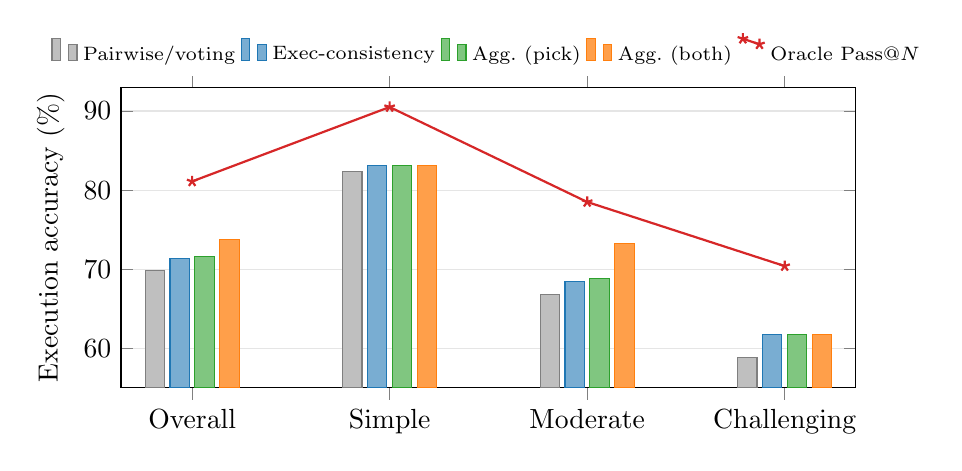
\begin{tikzpicture}
\begin{axis}[
  width=0.9\textwidth, height=5.4cm,
  ybar, bar width=7pt,
  enlarge x limits=0.12,
  ymin=55, ymax=93,
  ylabel={Execution accuracy (\%)},
  symbolic x coords={Overall,Simple,Moderate,Challenging},
  xtick=data,
  legend style={at={(0.5,1.20)},anchor=north,legend columns=5,font=\scriptsize,draw=none},
  ymajorgrids, grid style={gray!20},
]
\addplot[fill=axgray!50,draw=axgray] coordinates {(Overall,69.8)(Simple,82.4)(Moderate,66.8)(Challenging,58.8)};
\addplot[fill=axblue!60,draw=axblue] coordinates {(Overall,71.4)(Simple,83.1)(Moderate,68.4)(Challenging,61.8)};
\addplot[fill=axgreen!60,draw=axgreen] coordinates {(Overall,71.6)(Simple,83.1)(Moderate,68.8)(Challenging,61.8)};
\addplot[fill=axorange!75,draw=axorange] coordinates {(Overall,73.8)(Simple,83.1)(Moderate,73.2)(Challenging,61.8)};
\addplot[draw=axred,thick,sharp plot,mark=star,mark options={axred}] coordinates {(Overall,81.1)(Simple,90.5)(Moderate,78.5)(Challenging,70.4)};
\legend{Pairwise/voting, Exec-consistency, Agg.\ (pick), Agg.\ (both), Oracle Pass@$N$}
\end{axis}
\end{tikzpicture}
\caption{\textbf{Agentic aggregation vs.\ the oracle ceiling on BIRD mini-dev} (Qwen3-Coder-30B-A3B; visualizes Table~\ref{tab:agg}). The persistent gap between the best bar and the oracle star line is the ``selection gap,'' largest on \emph{moderate} and \emph{challenging} queries.}
\label{fig:agg}
\end{figure}

\begin{figure}[h]
\centering
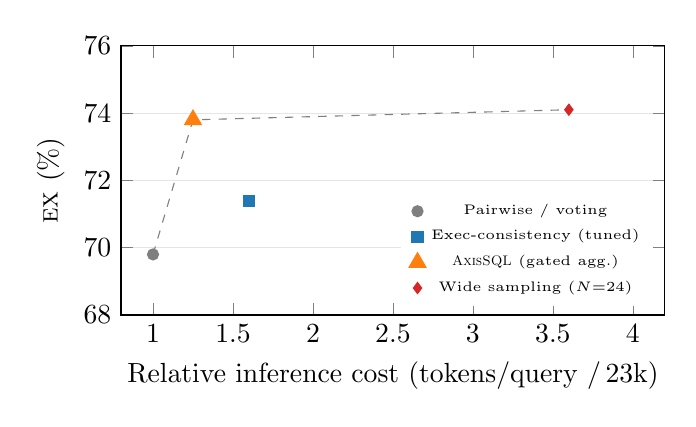
\begin{tikzpicture}
\begin{axis}[
  width=0.7\textwidth, height=5.0cm,
  xlabel={Relative inference cost (tokens/query $/\,23$k)},
  ylabel={\ex (\%)},
  xmin=0.8,xmax=4.2, ymin=68, ymax=76,
  ymajorgrids, grid style={gray!20},
  legend style={at={(0.98,0.03)},anchor=south east,font=\tiny,draw=none},
]
\addplot[only marks,mark=*,axgray] coordinates {(1.0,69.8)}; \addlegendentry{Pairwise / voting}
\addplot[only marks,mark=square*,axblue] coordinates {(1.6,71.4)}; \addlegendentry{Exec-consistency (tuned)}
\addplot[only marks,mark=triangle*,axorange,mark size=3.5pt] coordinates {(1.25,73.8)}; \addlegendentry{\sys{} (gated agg.)}
\addplot[only marks,mark=diamond*,axred] coordinates {(3.6,74.1)}; \addlegendentry{Wide sampling ($N{=}24$)}
\draw[dashed,gray] (axis cs:1.0,69.8) -- (axis cs:1.25,73.8) -- (axis cs:3.6,74.1);
\end{axis}
\end{tikzpicture}
\caption{\textbf{Accuracy vs.\ cost on BIRD mini-dev} (Qwen3-Coder; cost normalized to the $\sim$23k tokens/query pairwise baseline of \citealp{li2026deepeye}; referenced from Section~\ref{sec:main}). Confidence-gated aggregation (orange) is Pareto-optimal: it captures nearly all of the accuracy of much wider sampling (red) at $\sim$1.25$\times$ cost. The exec-consistency point (blue) is dominated.}
\label{fig:pareto}
\end{figure}

\begin{figure}[h]
\centering
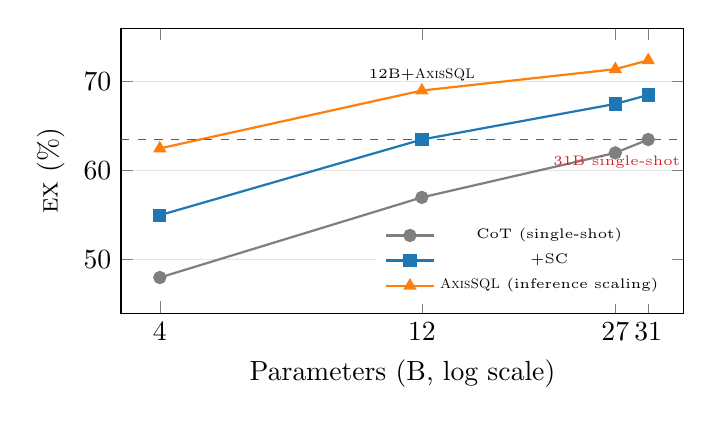
\begin{tikzpicture}
\begin{axis}[
  width=0.72\textwidth, height=5.2cm,
  xlabel={Parameters (B, log scale)},
  ylabel={\ex (\%)},
  xmode=log, log basis x=10,
  xmin=3.4, xmax=36, ymin=44, ymax=76,
  xtick={4,12,27,31}, xticklabels={4,12,27,31},
  legend style={at={(0.98,0.03)},anchor=south east,font=\tiny,draw=none},
  ymajorgrids, grid style={gray!20},
]
\addplot[axgray,thick,mark=*] coordinates {(4,48.0)(12,57.0)(27,62.0)(31,63.5)};
\addplot[axblue,thick,mark=square*] coordinates {(4,55.0)(12,63.5)(27,67.5)(31,68.5)};
\addplot[axorange,thick,mark=triangle*] coordinates {(4,62.5)(12,69.0)(27,71.4)(31,72.4)};
\draw[dashed,axred] (axis cs:3.4,63.5) -- (axis cs:36,63.5);
\node[axred,font=\tiny,anchor=west] at (axis cs:20,61.0) {31B single-shot};
\node[font=\tiny,anchor=south] at (axis cs:12,69.0) {12B$+$\sys};
\legend{CoT (single-shot), $+$SC, \sys{} (inference scaling)}
\end{axis}
\end{tikzpicture}
\caption{\textbf{Inference scaling shifts the parameter curve up, it does not flatten it} (Gemma-4 family; visualizes Table~\ref{tab:family}, referenced from Section~\ref{sec:family}). The $12$B$+$\sys{} point clears the red line ($31$B single-shot), so inference scaling on a small model beats a $2.6\times$ larger one run once---but at equal scaling the larger model stays ahead.}
\label{fig:family}
\end{figure}

\end{document}
